% Figure 1: MLAV platform, three layers and trust levels T0-T2. Compile: pdflatex fig1_architecture.tex
\documentclass[tikz,border=2pt]{standalone}
\usepackage{mathptmx}
\usetikzlibrary{positioning,fit,arrows.meta,backgrounds,calc}
\definecolor{okblue}{HTML}{0072B2}
\definecolor{okorange}{HTML}{E69F00}
\definecolor{okgreen}{HTML}{009E73}
\definecolor{okverm}{HTML}{D55E00}
\begin{document}
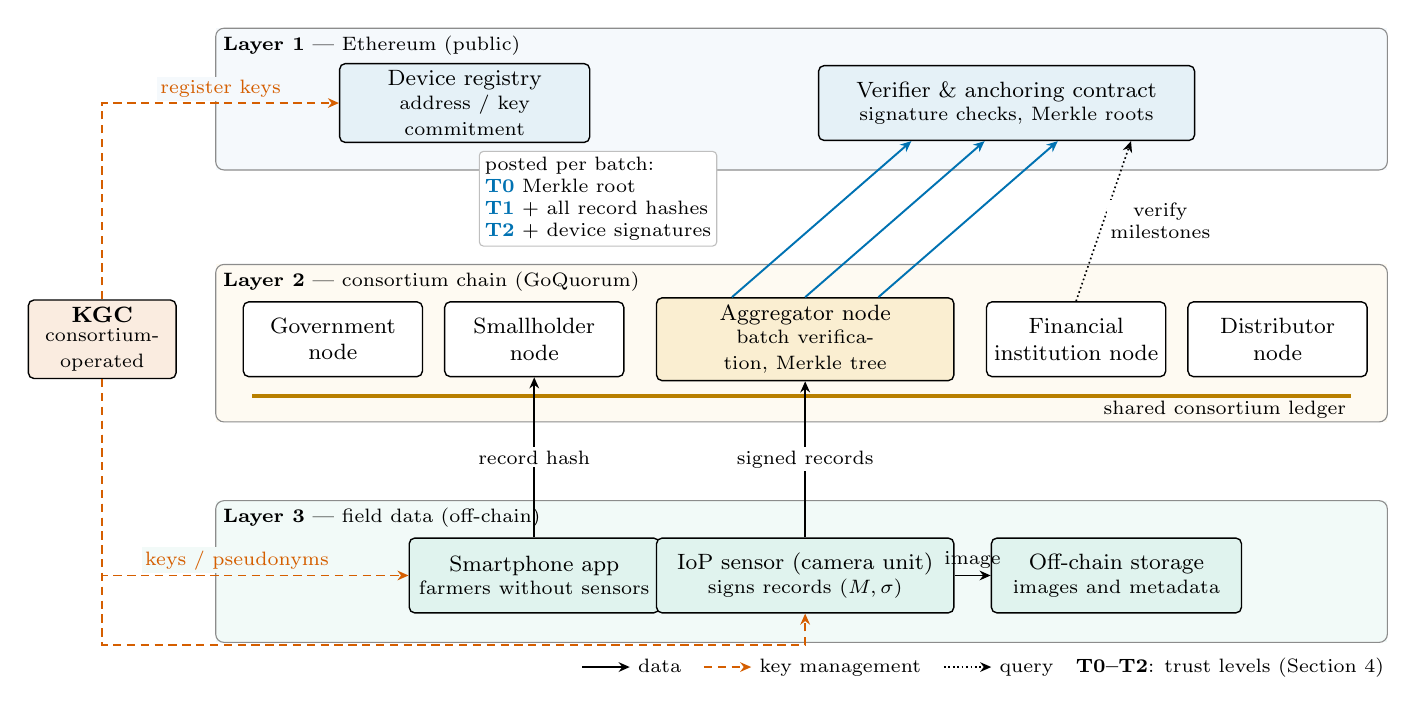
\begin{tikzpicture}[xscale=0.93,
  font=\footnotesize, >={Stealth[length=4pt,width=3.5pt]},
  box/.style={draw, rounded corners=2pt, align=center, minimum height=9.5mm, inner sep=2.5pt, fill=white, line width=0.5pt, text width=#1},
  box/.default=25mm,
  band/.style={draw=black!45, line width=0.4pt, rounded corners=3pt},
  lab/.style={font=\scriptsize, align=center, fill=white, inner sep=1.2pt},
  flow/.style={->, line width=0.7pt},
  ctrl/.style={->, line width=0.6pt, densely dashed, okverm},
]
% ---------------------------------------------------------------- coordinates (cm)
\def\yA{0}      % layer 1
\def\yB{-3.0}   % layer 2
\def\yC{-6.0}   % layer 3
\def\xL{-0.4}   % band left
\def\xR{15.6}   % band right

% ---------------------------------------------------------------- bands
\fill[okblue!4]   (\xL,\yA+0.95) rectangle (\xR,\yA-0.85);
\fill[okorange!5] (\xL,\yB+0.95) rectangle (\xR,\yB-1.05);
\fill[okgreen!5]  (\xL,\yC+0.95) rectangle (\xR,\yC-0.85);
\draw[band] (\xL,\yA+0.95) rectangle (\xR,\yA-0.85);
\draw[band] (\xL,\yB+0.95) rectangle (\xR,\yB-1.05);
\draw[band] (\xL,\yC+0.95) rectangle (\xR,\yC-0.85);
\node[anchor=north west, inner sep=2.5pt, font=\scriptsize] at (\xL,\yA+0.95) {\textbf{Layer 1} --- Ethereum (public)};
\node[anchor=north west, inner sep=2.5pt, font=\scriptsize] at (\xL,\yB+0.95) {\textbf{Layer 2} --- consortium chain (GoQuorum)};
\node[anchor=north west, inner sep=2.5pt, font=\scriptsize] at (\xL,\yC+0.95) {\textbf{Layer 3} --- field data (off-chain)};

% ---------------------------------------------------------------- layer 1
\node[box=30mm, fill=okblue!10] (reg) at (3.0,\yA) {Device registry\\[-1pt]{\scriptsize address / key commitment}};
\node[box=46mm, fill=okblue!10] (ver) at (10.4,\yA) {Verifier \& anchoring contract\\[-1pt]{\scriptsize signature checks, Merkle roots}};

% ---------------------------------------------------------------- layer 2
\node[box=21mm] (gov) at (1.2,\yB) {Government\\node};
\node[box=21mm] (sml) at (3.95,\yB) {Smallholder\\node};
\node[box=36mm, fill=okorange!18] (agg) at (7.65,\yB) {Aggregator node\\[-1pt]{\scriptsize batch verification, Merkle tree}};
\node[box=21mm] (fin) at (11.35,\yB) {Financial\\institution node};
\node[box=21mm] (dis) at (14.1,\yB) {Distributor\\node};
\draw[line width=1.4pt, okorange!80!black] (0.1,\yB-0.72) -- (15.1,\yB-0.72);
\node[font=\scriptsize, anchor=north east, inner sep=1.5pt] at (15.1,\yB-0.72) {shared consortium ledger};

% ---------------------------------------------------------------- layer 3
\node[box=30mm, fill=okgreen!12] (app) at (3.95,\yC) {Smartphone app\\[-1pt]{\scriptsize farmers without sensors}};
\node[box=36mm, fill=okgreen!12] (iop) at (7.65,\yC) {IoP sensor (camera unit)\\[-1pt]{\scriptsize signs records $(M,\sigma)$}};
\node[box=30mm, fill=okgreen!12] (sto) at (11.9,\yC) {Off-chain storage\\[-1pt]{\scriptsize images and metadata}};

% ---------------------------------------------------------------- KGC (outside the layers)
\node[box=17mm, fill=okverm!12] (kgc) at (-1.95,\yB) {\textbf{KGC}\\[-1pt]{\scriptsize consortium-\\operated}};

% ---------------------------------------------------------------- data flows
\draw[flow] (iop.north) -- node[lab] {signed records} (agg.south);
\draw[flow] (iop.east) -- node[lab, above=1pt, fill=none] {image} (sto.west);
\draw[flow] (app.north) -- node[lab] {record hash} (sml.south);
% aggregator -> Ethereum, one arrow per trust level
\draw[flow, okblue] ([xshift=-10mm]agg.north) -- ([xshift=-13mm]ver.south);
\draw[flow, okblue] (agg.north) -- ([xshift=-3mm]ver.south);
\draw[flow, okblue] ([xshift=10mm]agg.north) -- ([xshift=7mm]ver.south);
\node[lab, fill=white, draw=black!25, rounded corners=1.5pt, anchor=east, align=left, inner sep=2pt] at ([xshift=-12mm,yshift=12.5mm]agg.north) {%
  posted per batch:\\
  \textcolor{okblue}{\textbf{T0}} Merkle root\\
  \textcolor{okblue}{\textbf{T1}} + all record hashes\\
  \textcolor{okblue}{\textbf{T2}} + device signatures};
\draw[->, line width=0.6pt, densely dotted] (fin.north) -- node[lab, fill=white, right=1pt] {verify\\milestones} ([xshift=17mm]ver.south);

% ---------------------------------------------------------------- KGC control flows
\draw[ctrl] (kgc.north) |- node[lab, fill=okblue!4, pos=0.75, above=0.5pt] {register keys} (reg.west);
\draw[ctrl] (kgc.south) |- node[lab, fill=okgreen!5, pos=0.72, above=0.5pt] {keys / pseudonyms} (app.west);
\draw[ctrl] (kgc.south) |- ([yshift=-4mm]iop.south) -- (iop.south);

% ---------------------------------------------------------------- legend
\node[anchor=north east, font=\scriptsize, inner sep=1pt] at (\xR,\yC-1.0) {%
\tikz[baseline=-0.6ex]\draw[flow] (0,0)--(6mm,0); data\quad
\tikz[baseline=-0.6ex]\draw[ctrl] (0,0)--(6mm,0); key management\quad
\tikz[baseline=-0.6ex]\draw[->, line width=0.6pt, densely dotted] (0,0)--(6mm,0); query\quad
\textbf{T0--T2}: trust levels (Section~4)};
\end{tikzpicture}
\end{document}
